\documentclass{article}
\usepackage{graphicx} % Required for inserting images
\usepackage{amsmath}
\usepackage{mathtools}
\usepackage[utf8]{inputenc}
\usepackage{amssymb}
\usepackage{amsthm}
\usepackage{url}
\usepackage{hyperref}
\usepackage{xcolor}
\usepackage[linguistics]{forest}
\usepackage{lineno}
\usepackage{tikz}
\usetikzlibrary{automata, positioning}

\title{Theoretische Informatik II}
\date{}

\hypersetup{
	colorlinks=true,
	linkcolor=teal,
	filecolor=magenta,      
	urlcolor=cyan,
}

% Benutzt, um \wedge als großes Symbol für die Iteration zu benutzen
\def\Wedgeop{\operatornamewithlimits{%
		\mathchoice{\vcenter{\hbox{\huge $\wedge$}}}
		{\vcenter{\hbox{\Large $\wedge$}}}
		{\mathrm{A}}
		{\mathrm{A}}}}

% Benutzt, um \vee als großes Symbol für die Iteration zu benutzen
\def\Veeop{\operatornamewithlimits{%
		\mathchoice{\vcenter{\hbox{\huge $\vee$}}}
		{\vcenter{\hbox{\Large $\vee$}}}
		{\mathrm{A}}
		{\mathrm{A}}}}

\newcommand*\conj[1]{\bar{#1}}
\newcommand*\mean[1]{\bar{#1}}
\newcommand\myeq{\stackrel{\mathclap{\normalfont\mbox{IV}}}{=}}
\newcommand\griv{\stackrel{\mathclap{\normalfont\mbox{IV}}}{>}}
\newcommand\phut{\stackrel{\mathclap{\normalfont\mbox{^}}}{P}}

% Da fängt's wieder an

\begin{document}
	% Erstelle das Inhaltsverzeichnis
	\maketitle
	\tableofcontents
	\newpage
	
	\section{Aussagenlogik}
	\textcolor{gray}{Einheit 1 und 2 aus Vorlesung Nr.1} \\
	
	\subsection{Syntax der Aussagenlogik}
	\begin{itemize}
		\item Atomare Formeln $(A_i, i =1,2,3)$ sind Formeln.\\
		\textcolor{gray}{Atomare Formeln sind einfache Aussagen wie "Der Himmel ist Blau"}
		\item Falls $F$ und $G$ Formeln sind, dann sind auch $(F \wedge G)$, $(F \vee G)$, $(F \Rightarrow G)$ und $(F \Leftrightarrow G)$ Formeln.
		\item Wenn $F$ eine Formel ist, dann ist auch $\neg F$ eine Formel
	\end{itemize}
	
	\subsection{Abkürzungen}
	\begin{itemize}
		\item Namen ohne Index: $A, B, C, ...$ für $A_1, A_2, A_3, ...$\\
		\textcolor{gray}{In dem Fall $A = A_1; B = A_2; C = A_3; ...$}
		\item Implikation \textcolor{red}{$F_1 \rightarrow F_2$}	steht für $(\neg F_1 \vee F_2)$
		\item Äquivalenz \textcolor{red}{$F_1 \leftrightarrow F_2$}		steht für $((F_1 \wedge F_2) \vee (\neg F_1 \wedge \neg F_2))$ 
		\item n-Faches Oder \[\Veeop^{n}_{i = 1} F_i\] 
		steht für $(...((F_1 \vee F_2)\vee F_3)... \vee F_n)$
		\item n-Faches Und \[\Wedgeop^n_{i=1} F_i\]
		steht für $(...((F_1 \wedge F_2)\wedge F_3)... \wedge F_n)$
	\end{itemize}
	
	Beispiel:
	\begin{align*}
		B \leftrightarrow (C \rightarrow E) &= ((B \wedge A)\vee(\neg B \wedge \neg A)) \: [1]\\
		&= ((B \wedge (C \rightarrow E))\vee(\neg B \wedge \neg (C \rightarrow E))) \: [2] \\
		&= ((B \wedge (\neg C \vee E))\vee(\neg B \wedge \neg (\neg C \vee E))) \: [3]\\
		&= ((A_2 \wedge (\neg A_3 \vee A_5))\vee(\neg A_2 \wedge \neg (\neg A_3 \vee A_5))) \: [4]
	\end{align*}
	\textcolor{gray}{
		$[1]$ Äquivalenzformel angewendet und $A = C \rightarrow E$ \\
		$[2]$ $A$ mit $C \rightarrow E$ ersetzt \\
		$[3]$ Implikationsformel angewendet \\
		$[4$] Namen ohne Index angewendet aber andersherum
	}
	
	\subsection{Semantik der Aussagenlogik}
	Sei $D$ eine Teilmenge von Formeln $\{A_1, A_2, ...\}$. \\
	Eine Abbildung $\mathcal{A}: D \rightarrow \{0,1\}$ heißt \textbf{Belegung}.\\ 
	\\
	\textcolor{gray}{Die Elemente in $\{0,1\}$ heißen die \textbf{Wahrheitswerte}. Man schreibt 0 statt falsch und 1 statt wahr.}  \\
	\\
	Durch eine Belegung erhält jede atomare Formel einen Wert. 
	\begin{itemize}
		\item \textbf{Induktionsanfang:} \\
		Der Wert einer atomaren Formel $A_i$ ist genau dann definiert, wenn $A_i \in D$ gilt, und er ist dann $\mathcal{A}(A_i)$.
		\item \textbf{Induktionsschritt:} \\
		Wir nehmen an, dass $\mathcal{A}(F)$ und $\mathcal{A}(G)$ definiert sind.
		\begin{itemize}
			\item $\mathcal{A}(F \wedge G)$ sei das Minimum von $\mathcal{A}(F)$ und $\mathcal{A}(G)$ \\
			\textcolor{gray}{$\mathcal{A}(F \wedge G) = 1 \leftrightarrow \mathcal{A}(F) = 1 \wedge \mathcal{A}(G) = 1$}
			\item $\mathcal{A}(F \vee G)$ sei das Maximum von $\mathcal{A}(F)$ und $\mathcal{A}(G)$ \\
			\textcolor{gray}{$\mathcal{A}(F \wedge G) = 1 \leftrightarrow \mathcal{A}(F) = 1 \vee \mathcal{A}(G) = 1$}
			\item $\mathcal{A}(\neg F)$ sei definiert durch $\mathcal{A}(\neg F) = 1 - \mathcal{A}(F)$
			\textcolor{gray}{$\mathcal{A}(\neg F) \leftrightarrow \mathcal{A}(F) = 0$}
		\end{itemize}
	\end{itemize}
	\subsection{Verknüpfungstabellen}
	\begin{tabular}{|c|c|c|}
		\hline
		$\mathcal{A}(F)$ & $\mathcal{A}(G)$ & $\mathcal{A}(F \rightarrow G)$ \\
		\hline
		0 & 0 & 1 \\
		0 & 1 & 1 \\
		1 & 0 & 0 \\
		1 & 1 & 1 \\
		\hline
	\end{tabular}
		\begin{tabular}{|c|c|c|}
		\hline
		$\mathcal{A}(F)$ & $\mathcal{A}(G)$ & $\mathcal{A}(F \leftrightarrow G)$ \\
		\hline
		0 & 0 & 1 \\
		0 & 1 & 0 \\
		1 & 0 & 0 \\
		1 & 1 & 1 \\
		\hline
	\end{tabular}
	\subsection{Baumstruktur für Formeln}
	\begin{enumerate}
		\item Für atomare Formeln wird ein Knoten, in den als Label die atomare Formel eingetragen: \\
		\\ % Es wird ein Automat benutzt, um einfach den Kreis um den Label zu haben
			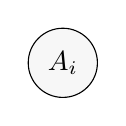
\begin{tikzpicture}[shorten >=1pt,node distance=2cm,on grid,auto]
			\tikzstyle{every state}=[fill={rgb:black,1;white,30}]
			
			\node[state] (0) at (0,0) {$A_i$};
		\end{tikzpicture}
		\\
		\\
		\\
		\\ % Damit der neue Punkt mit dem "Automaten" verbunden ist
		\\ % Hier wird immernoch ein "Automat" benutzt, um 
		\\ % die coolen Kreise zu haben
		\\
		\item Für $\neg F$ wird ein Knoten, in den als Label die Verknüpfung eingetragen ist, darunter ein Baum $B$ für $F$: \\
		\\
		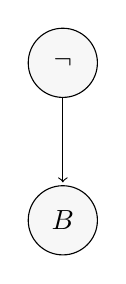
\begin{tikzpicture}[shorten >=1pt,node distance=2cm,on grid,auto]
			\tikzstyle{every state}=[fill={rgb:black,1;white,30}]
			
			\node[state] (q_0) at (0,2) {$\neg$};
			\node[state] (q_1) at (0,0){$B$};
			
			\path[->]
			(q_0) edge node { } (q_1);
		\end{tikzpicture}
		\\
		\\
		\textcolor{gray}{In dem Fall ist $B$ der Baum für $F$. \\
		Man kann das so allgemeinern, weil z.B kann $F$ auch $A_1 \leftrightarrow A_2$ sein.
		}
		\item Für $F \wedge G$ wird ein Knoten, in den als Label $\wedge$ eingetragen ist, darunter Bäume für $F$ und $G$: 
		\\
		\\
		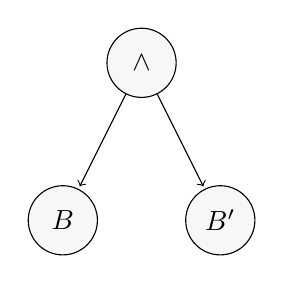
\begin{tikzpicture}[shorten >=1pt,node distance=2cm,on grid,auto]
			\tikzstyle{every state}=[fill={rgb:black,1;white,30}]
			
			\node[state] (q_0) at (2,2) {$\wedge$};
			\node[state] (q_1) at (1,0){$B$};
			\node[state] (q_2) at (3,0){$B'$};
					
			\path[->]
			(q_0) edge node { } (q_1)
			(q_0) edge node { } (q_2);
		\end{tikzpicture}
		\\
		\\
		\textcolor{gray}{Analog zu Punkt 2. ist $B$ ein Baum für $F$ und $B'$ ein Baum für $G$.} \\
		\\
		Das gleiche gilt auch für $\vee$. \\
		\\
		Beispiel von einer Baumstruktur: \\
		Formel: $((A\wedge(B\vee C))\vee(\neg A \wedge (B \vee C)))$ \\
		\\
		\begin{forest}
			[ $\vee$ 
			 [$\wedge$ 
			 	[A]
			 	[$\vee$
			 		[B]
			 		[C]
			 	]
			 ]
			 [$\wedge$ 
			 	[$\neg$ 
			 		[A]
			 	]
			 		[$\vee$
			 			[B]
			 			[C]
			 		]
			 ]
			]
		\end{forest}
		\\
		Man wertet den Syntaxbaum von unten nach oben ab.
	\end{enumerate}
	\subsection{Modelle, Gültigkeit, Erfüllbarkeit und Tautologie}
	Sei $F$ eine Formel und sei $\mathcal{A} : M \rightarrow \{0,1\}$ eine Belegung. \\
	\textcolor{gray}{$M$ ist hierbei die Teilmenge der Formeln.}
	\begin{itemize}
		\item Sind alle in $F$ vorkommenden atomaren Formeln im Definitionsbereich von $\mathcal{A}$ enthalten, so heißt $\mathcal{A}$ zu $F$ \textbf{passend}.\\
		\textcolor{gray}{Sei $F = A \wedge B$ mit $\mathcal{A}(A) \in \{0,1\}$, dann ist $F$ passend.}
		\item Ist $\mathcal{A}$ zu $F$ passend und gilt $\mathcal{A}(F) = 1$, so schreiben wir $\mathcal{A} \vDash F$. Wir sagen, dass $F$ unter der Belegung $\mathcal{A}$ gilt und nennen $\mathcal{A}$ ein \textbf{Modell} für $F$.
		\item Ist $\mathcal{F}$ eine Menge von Formeln, so heißt $\mathcal{A}$ ein \textbf{Modell} für $\mathcal{F}$, wenn für alle $F \in \mathcal{F}$ gilt: $\mathcal{A} \vDash F$. In diesem Fall wird dann $\mathcal{A} \vDash \mathcal{F}$ geschrieben. \\
		\textcolor{gray}{Aufgeteilt: Falls alle Formeln in $\mathcal{F}$ die Bedingung "$\mathcal{A}$ ist passend zu $F$" und die Bedingung "$\mathcal{A}(F)=1$" für alle $F \in \mathcal{F}$ erfüllt, dann ist $\mathcal{A}$ ein Modell für $\mathcal{F}$}
		\item $F$ ist \textbf{erfüllbar}, wenn es ein Modell für $F$ gibt. \\
		\textcolor{gray}{Es existiert eine Belegung $\mathcal{A}$, die zu $F$ passend ist, mit $\mathcal{A}(F) = 1$.}
		\item $F$ ist \textbf{gültig}, falls für alle $\mathcal{A}$, die zu $F$ passend sind, $\mathcal{A}(F) = 1$ gilt.
		\item Eine \textbf{Tautologie} ist eine gültige Formel $F$.
	\end{itemize}
	\subsection{Zusammenhang Erfüllbarkeit/Tautologie}
	\[F \:\: ist \:\: Tautologie \Leftrightarrow \neg F \:\: ist \:\: unerf\ddot{u}llbar\]
	\subsection{Das Spiegelungsprinzip}
	\begin{itemize}
		\item Gültige Formeln werden durch Negation zu unerfüllbaren Formeln. 
		\item Unerfüllbare Formeln werden durch Negation zu gültigen Formeln.
		\item Erfüllbare, nicht gültige Formeln werden durch Negation wieder zu erfüllbaren, nicht gültigen Formeln.
	\end{itemize}
	\subsection{Wahrheitswerteverlauf}
	Der Wahrheitswert von $F$ unter passender Belegung $\mathcal{A}$ hängt \textbf{nur} vom Wahrheitswert der atomaren Formeln in $F$ ab. \\
	Dadurch kann man Erfüllbarkeit, Gültigkeit und ähnliche Eigenschaften bei $F$ testen, indem man Wahrheitstabellen erstellt. \\
	\\
	Für die Spalten setzt man $A_1, ..., A_n$ und $F$ ein. \\
	\textcolor{gray}{Anzahl der Spalten ist die Anzahl aller Teilformeln von F} \\
	Für die Zeilen setzt man $A_i$ mit $i = 1, ..., 2^n$ \\
	\textcolor{gray}{Anzahl der Zeilen ist $2^{Anzahl \: atomare \: Formeln}$}\\
	\\
	\textbf{Beispiel:} \\
	\textcolor{gray}{In dem Fall hat $\equiv$ die gleiche Bedeutung wie $\Leftrightarrow$, aber es wird später mehr erläutert.} \\
	$F:= (A \wedge B) \equiv (B \wedge A)$ \\
	\\
	Wahrheitstabelle \\
	\\
	\begin{tabular}{|c|c|c|c|c|c|}
		\hline
		Belegung $\mathcal{A}$ & A & B & $A \wedge B$ & $B \wedge A$ & $A \wedge B \equiv B \wedge A$ \\ 
		\hline
		1 & 0 & 0 & 0 & 0 & 1 \\
		\hline
		2 & 0 & 1 & 0 & 0 & 1 \\
		\hline
		3 & 1 & 0 & 0 & 0 & 1 \\
		\hline
		4 & 1 & 1 & 1 & 1 & 1 \\
		\hline
	\end{tabular}
	\\
	\\
	\textcolor{gray}{Jede einzelne Zeile entspricht einer Belegung $\mathcal{A}$} \\
	\textcolor{gray}{\textbf{Teilformel}: Eine Formel, die in $F$ ist. Nach Definition sind atomare Formeln Formeln und alle Verknüpfungen zwischen 2 atomaren Formeln auch Formeln.}
	\begin{itemize}
		\item Alle $\mathcal{A}$ sind zu F passend, weil alle atomaren Formeln im Definitionsbereich von $\mathcal{A}$ liegen.
		\item Bei der ersten Belegung ist $\mathcal{A}$ ein Modell für F, weil $\mathcal{A}$ passend zu F ist und $\mathcal{A}(F)=1$ gilt. \\
		$\Rightarrow F$ ist erfüllbar.
		\item Bei allen Belegungen $\mathcal{A}$ gilt, dass alle $\mathcal{A}$ passend zu F ist und $\mathcal{A}(F) = 1$ gilt.  \\
		$\Rightarrow F$ ist gültig und eine Tautologie.
	\end{itemize}
	\subsection{Äquivalenz aussagenlogischer Formeln}
	$F$ und $G$ heißen \textbf{semantisch äquivalent}, wenn für alle zu beiden passenden Belegungen $\mathcal{A}$ gilt: 
	\[\mathcal{A}(F) = \mathcal{A}(G)\]
	In diesem Fall schreiben wir $F \equiv G$.
	\subsection{Das Ersetzbarkeitstheorem}
	Sei $H$ eine Formel, in der $F$ als Teilformel vorkommt. \\
	Sei $G$ eine zu $F$ äquivalente Formel. \\
	Sei $H'$ die Formel, die aus $H$ entsteht, wenn $F$ durch $G$ ersetzt wird. \\
	Dann sind $H$ und $H'$ äquivalent. \\
	\textcolor{gray}{Äquivalentes Ersetzen von Teilformeln erhält Äquivalenz!} \\
	\\
	\\
	\\
	\\
	\textbf{Beispiel: }\\
	\begin{align*}
		\delta &= (B \rightarrow (A \wedge (A \vee B))) \\
		\alpha &= (A \wedge (A \vee B)) \\
		\beta &= A \\
		\delta' &= (B \rightarrow A)
	\end{align*}
	\begin{align*}
		\delta &= (B \rightarrow (A \wedge (A \vee B))) \: [1] \\
	    	   &= (B \rightarrow \textcolor{teal}{\alpha}) \: [2]  \\
	    	   &= (B \rightarrow \textcolor{teal}{\beta}) \: [3] \\
	    	   &= (B \rightarrow \textcolor{teal}{A})\\
	    	   &= \delta'
	\end{align*}
	\textcolor{gray}{
		$[1]$ Formel eingesetzt.\\
		$[2]$ $\alpha$ eingesetzt, weil es gleich ist.\\
		$[3]$ Da $\alpha \equiv \beta$ (Beweis durch Wahrheitstabelle), wird $\alpha$ durch $\beta$ ersetzt.\\
	}
	\section{Normalformen der Aussagenlogik}
	\textcolor{gray}{Einheit 3 aus Vorlesung Nr.2}
	\subsection{Äquivalenzen}
	\begin{itemize}
		\item \textbf{Idempotenz: }\\
		\[F \equiv (F \wedge F) \equiv (F \vee F)\]
		\item \textbf{Kommutativität: }\\
		\[(F\wedge G) \equiv (G \wedge F) \quad (F \vee G) \equiv (G \vee F)\]
		\item \textbf{Assoziativität:} \\
		\[((F \wedge G) \wedge H) \equiv (F \wedge (G \wedge H))\]
		\[((F \vee G) \vee H) \equiv (F \vee (G \vee H))\]
		\item \textbf{Absorption:} \\
		\[(F \wedge (F \vee G)) \equiv F \equiv (F \vee (F \wedge G))\]
		\item \textbf{Distributivität:}\\
		\[(F \wedge (G \vee H)) \equiv ((F \wedge G) \vee (F \wedge H))\]
		\[(F \vee(G \wedge H)) \equiv ((F \vee G) \wedge (F \vee H)) \]
		\item \textbf{Doppelnegation:}\\
		\[\neg\neg F \equiv F\]
		\item \textbf{deMorgan-Regeln:}\\
		\[\neg(F \wedge G)\equiv (\neg F \vee \neg G) \quad \neg(F \vee G) \equiv (\neg F \wedge \neg G)\]
		\item \textbf{Tautologie:}\\
		Falls F eine Tautologie ist, gelten folgende Äquivalenzen: \\
		\[(F \vee G) \equiv F \quad (F \wedge G) \equiv G\]
		\item \textbf{Unerfüllbarkeit:}\\
		Falls F unerfüllbar ist, dann gelten folgende Äquivalenzen:\\
		\[(F \vee G) \equiv G \quad (F \wedge G) \equiv F\]
		\subsection{Assoziativität und Klammerung}
		Man darf sich erlauben, Klammerungen bei zusammengesetzten $\wedge$ oder $\vee$ Formeln (bzw. Teilformeln) wegzulassen. \\
		\\
		\textbf{Beispiel:} \\
		Wir schreiben $A \vee B \vee C$ sowohl für $((A \vee B) \vee C)$ als auch für $(A \vee (B \vee C))$ \\
		\\
		\textbf{Wichtig:} \\
		Nicht zu viele Klammern wegmachen! \\
		Was würde dann bei $A \wedge B \vee C$ passieren? \\
		\subsection{Normalformen}
		\begin{itemize}
			\item Ein \textbf{positives Literal} ist eine atomare Formel.
			\item Ein \textbf{negatives Literal} ist die Negation einer atomaren Formel.
		\end{itemize} 
		\textbf{Definitionen:}
		\begin{itemize}
			\item Eine Formel F ist in disjunkter Normalform (DNF), wenn sie eine Disjunktion von Konjunktionen von Literalen ist.
			\item Die Formel F ist in konjunktiver Normalform (KNF), wenn sie eine Konjunktion von Disjunktionen von Literalen ist
		\end{itemize}
		\subsection{Satz (DNF/KNF)}
		Zu jeder Formel existieren äquivalente Formeln in DNF und in KNF.
		\subsection{KNF-Algorithmus}
		\begin{enumerate}
			\item Negationen nach innen schieben (deMorgan-Regeln) und dabei Doppelnegationen eliminieren.
			\item Zweites Distibutivgesetz nutzen, um $\vee$-Operationen vorbei nach innen zu schieben.
		\end{enumerate}
		\textcolor{gray}{Dabei wird die Ausgangsformel nur mit $\neg$, $\vee$ und $\wedge$ gebildet.} \\
		\\
		\textbf{Beispiel:} \\
		\begin{align*}
			(\neg(A \wedge\neg(C \vee \neg B))\vee \neg(\neg D \vee (B \wedge A))) 
			\equiv& (\neg(A \wedge\textcolor{teal}{(\neg C \wedge B)}) \vee \textcolor{teal}{(D \wedge \neg (B \wedge A))}) \: [1] \\
			\equiv& \textcolor{teal}{((\neg A \vee (C \vee \neg B))} \vee (D \wedge \textcolor{teal}{(\neg B \vee \neg A)})) \: [2] \\
			\equiv& (\neg A \vee C \vee \neg B \vee D) \wedge (\neg A \vee C \vee \neg B \vee \neg B \vee \neg A) \: [3]
		\end{align*}
		Dabei ist die letzte Formel in KNF. \\
		\textcolor{gray}{
			$[1]$ deMorgansche-Regeln bei beiden. (Doppelnegierungen werden weggestrichen)\\
			$[2]$ deMorgansche-Regeln erneut.\\
			$[3]$ Da spielt das 2. Distributivgesetz eine große Rolle:
		}
		\begin{align*}
			((\neg A \vee (C \vee \neg B)) \vee (D \wedge (\neg B \vee \neg A))) &\equiv \textcolor{red}{(\neg A \vee C \vee \neg B)} \vee (\textcolor{blue}{D} \wedge \textcolor{green}{(\neg B \vee \neg A)}) \: [1] \\
			&\equiv (\neg A \vee C \vee \neg B \vee D) \wedge (\neg A \vee C \vee \neg B \vee \neg B \vee \neg A) \: [2]
		\end{align*}
		\textcolor{gray}{
			$[1]$ \textcolor{red}{Rot ist F}, \textcolor{blue}{Blau ist G} und \textcolor{green}{Grün ist H}. Dabei erhält man die Formel $(F \vee (G \wedge H))$ und diese ist äquivalent zu $((F \vee G) \wedge (F \vee H))$\\ (2. Distributivformel)\\
			$[2]$ Die Formel aus der Beschreibung von $[1]$ angewendet.\\
		}
		\subsection{KNF aus der Wahrheitstafel}
		\begin{tabular}{c|c|c||c}
			A & B & C & F \\
			\hline
			0 & 0 & 0 & 0 \\
			0 & 0 & 1 & 1 \\
			0 & 1 & 0 & 1 \\
			0 & 1 & 1 & 0 \\
			1 & 0 & 0 & 1 \\
			1 & 0 & 1 & 1 \\
			1 & 1 & 0 & 1 \\
			1 & 1 & 1 & 0 \\
		\end{tabular}
		\begin{enumerate}
			\item Betrachte alle Fälle, wo F gleich 0 ist. 
			\item Um eine Zeile mit Null zu "vermeiden", muss mindestens eine der atomaren Formeln den Wert 1 annehmen
			\item Wiederhole das alles auch bei den anderen Zeilen mit Null und verknüpfe sie mit $\wedge$
		\end{enumerate}
			Resultat: \\
			Aus Zeile 1: $(A \vee B \vee C)$ \\
			Aus Zeile 4: $(A \vee \neg B \vee \neg C)$ \\
			Aus Zeile 8: $(\neg A \vee \neg B \vee \neg C)$ \\
		Daraus ergibt sich 
		\[F \equiv F' = (A \vee B \vee C) \wedge (A \vee \neg B \vee \neg C) \wedge (\neg A \vee \neg B \vee \neg C)\]
		\subsection{DNF aus der Wahrheitstafel}
		\begin{tabular}{c|c|c||c}
			A & B & C & F \\
			\hline
			0 & 0 & 0 & 0 \\
			0 & 0 & 1 & 1 \\
			0 & 1 & 0 & 1 \\
			0 & 1 & 1 & 0 \\
			1 & 0 & 0 & 1 \\
			1 & 0 & 1 & 1 \\
			1 & 1 & 0 & 1 \\
			1 & 1 & 1 & 0 \\
		\end{tabular} \\
		\\
		Für den DNF muss man umgekehrt die positiven Fälle betrachten und mit $\vee$ verknüpfen. \\
		\\
		Also: \\
		Zeile 2: $(\neg A \wedge \neg B \wedge C)$ \\
		Zeile 3: $(\neg A \wedge B \wedge \neg C)$ \\
		Zeile 5: $(A \wedge \neg B \wedge \neg C)$ \\
		Zeile 6: $(A \wedge \neg B \wedge C)$ \\
		Zeile 7: $(A \wedge B \wedge \neg C)$ \\
		\\
		Damit erhält man die äquivalente Formel in DNF: \\
		$F \equiv F' = (\neg A \wedge \neg B \wedge C) \vee (\neg A \wedge B \wedge \neg C) \vee (A \wedge \neg B \wedge \neg C)$\\$ \vee (A \wedge \neg B \wedge C) \vee (A \wedge B \wedge \neg C)$
	\end{itemize}
	\section{Prädikatenlogik erster Stufe}
	\textcolor{gray}{Einheit 4 aus Vorlesung Nr.2}
	\subsection{Grundbegriffe der Prädikatenlogik}
	Die Aussagenlogik kann folgendes nicht ausdrücken:
	\begin{itemize}
		\item \textcolor{red}{Für alle} Objekte einer gewissen Art gilt ...
		\item \textcolor{red}{Es gibt} ein Objekt einer gewissen Art mit ...
		\item \textbf{Funktionen} und \textbf{Relationen}.
	\end{itemize}
	Deswegen gibt es die Prädikatenlogik (erster Stufe) \\
	\\
	Man verwendet drei Sorten von Objekten
	\begin{itemize}
		\item Eine \textbf{Variable} hat die Form $x_i$ für ein $i \in \{1,2,...\}$
		\item Ein \textbf{Prädikatsymbol} hat die Form $P^k_i$ für ein $i \in \{1,2,...\}$ und ein $k \in \{0,1,2,...\}$
		\item Ein \textbf{Funktionssymbol} hat die Form $f^k_i$ für ein $i \in \{1,2,...\}$ und ein $k \in \{0,1,2,...\}$
	\end{itemize}
	Dabei ist $i$ ein Index, der es ermöglicht, eine beliebige Anzahl dieser Objekte zu verwenden. $i$ heißt auch \textbf{Unterscheidungsindex}. \\
	$k$ ist die \textbf{Stelligkeit} oder Stellenzahl von $P^k_i$ bzw. $f^k_i$
	\subsection{Syntax der Prädikatenlogik}
	Die Menge der \textbf{Terme} wird so induktiv definiert
	\begin{itemize}
		\item Wenn P ein k-stelliges Prädikatensymbol ist und $t_1, ..., t_k$ Terme sind dann ist $P(t_1,...,t_k)$ eine \textbf{atomare Formel}.
		\item Mit F und G sind auch $\neg F$, $(F \wedge G)$ und $(F \vee G)$ Formeln
		\item Ist F eine Formel und x eine Variable, dann sind auch $\exists x F$ und $\forall x F$ Formeln
	\end{itemize}
	\subsection{Semantik der Prädikatenlogik}
	Zweck ist es, den benutzten Variablen, Funktionssymbolen und Prädikatsymbolen einen realen Sinn zuzuordnen. \\
	\\
	Dafür werden Individuen benutzt, also mögliche Werte für die Variablen und Terme,\\
	sowie eine Zuordnung der Funktions- und Prädikatsymbole zu realen Funktionen und Prädikaten.\\
	\\
	Prädikatenlogische Formeln wird mit einer Struktur interpretiert:
	\begin{itemize}
		\item Gegeben ist ein Paar $\mathcal{A} = (U_\mathcal{A}, I_\mathcal{A})$. \\
		\textcolor{gray}{Dabei ist das Paar $\mathcal{A}$ eine Struktur.}
		\item $U_\mathcal{A}$ heißt \textbf{Menge der Individuen}.
		\item $I_\mathcal{A}$ ist eine Abbildung, die jedem (in der Formel benutzen) Prädikatsymbol $P^k_i$ bzw. Funktionssymbol $f^k_i$ ein dazu passendes Prädikat/eine passende Funktion zuordnet, sowie jeder benutzten Variablen $x_i$ einen Wert aus $U_\mathcal{A}$.
	\end{itemize} 
	\textbf{Beispiele: }
	\begin{itemize}
		\item Aus welcher Menge kommt $I_\mathcal{A}(f^0_3())$? Lösung: $U_\mathcal{A}$ 
		\item Aus welcher Menge kommt $I_\mathcal{A}(P^3_4))$? Lösung: $\mathcal{P}(U_\mathcal{A} \times U_\mathcal{A} \times U_\mathcal{A})$
		\item Aus welcher Menge kommt $I_\mathcal{A}(f^2_3)$? Lösung: $U_\mathcal{A} \times U_\mathcal{A} \rightarrow U_\mathcal{A}$
	\end{itemize}
	\subsection{Beispiel für Strukturen/Werte von Termen}
	Man geht von einer gegebenen Formel aus, wie z.B:
	\[F = \forall x \exists y \exists y' ((P(x,y)\wedge P(x,y'))\wedge \forall z (\neg P(x,z)\vee(Q(y,z)\vee Q(y',z))))\]
	%\textcolor{gray}{Das ist nur ein Beispiel. Diese Formel wird nicht für's Erklären benutzt.}\\
	Als \textbf{Individuenbereich} $U_\mathcal{A}$ nimmt man häufig $\mathbb{N}$ - das muss aber nicht sein. \\
	Durch $I_\mathcal{A}$ müssen dann alle freien Variablen, Prädikate und alle Funktionen definiert werden. In dem Fall wählen wir jetzt \\
	\\
	$U_\mathcal{A} = V$ für einen ungerichteten Graphen $G = (V,E)$ \\
	$I_\mathcal{A}(P) = P^\mathcal{A} = \{(u,v) \:|\: u,v \in V \: und \: \{u,v\}\in E\}$ (Kantenrelation)\\
	$I_\mathcal{A}(Q) = Q^\mathcal{A} = \{(u,v) \:|\: u \in V\}$  (Gleichheit) \\
	\\
	Durch das Paar $\mathcal{A} = (U_\mathcal{A}, I_\mathcal{A})$ können nun allen Termen \textcolor{red}{Werte aus $U_\mathcal{A}$} zugewiesen werden wie folgt:
	\begin{itemize}
		\item Eine (freie) Variable $x_i$ erhält den Wert $I_\mathcal{A}(x_i)$
		\item Ein Term der Form $f^k_i(t_1,..., t_k)$ erhält den Wert $I_\mathcal{A}(f^k_i)(u_1,...,u_k)$ \\
		wenn die $t_i$ jeweils den Wert $u_i$ haben.
	\end{itemize}
	\textcolor{gray}{
		Den Wert des Terms $t$ in der Struktur $\mathcal{A}$ bezeichnet man mit $\mathcal{A}(t)$. \\
		Also: $\mathcal{A}(t) \in U_\mathcal{A}$ für alle Terme t.
	} \\
	\subsection{Wahrheitswerte von Formeln}
	Die atomare Formel $F = P(t_1, ..., t_k)$ ist wahr, falls $(\mathcal{A}(t_1),...,\mathcal{A}(t_k)) \in P^\mathcal{A}$ gilt. Wir schreiben dann $\mathcal{A}(F) = 1$. \\
	Andernfalls ist dann $\mathcal{A}(F) = 0$, bzw. F ist nicht wahr. \\
	\textcolor{gray}{
		Die Definitionen von $\mathcal{A}(\neg F)$, $\mathcal{A}(F \wedge G)$ und $\mathcal{A}(F \vee G)$ sind gleich zum aussagenlogischen Fall
	} \\
	\\
	\\
	Ist $F= \forall x G$, so definieren wir $\mathcal{A}(F)$ so: 
	\begin{itemize}
		\item $\mathcal{A}(F) = 1$, falls $\forall \alpha \in U_\mathcal{A}: \mathcal{A}_{[x/\alpha]}(G) = 1$
		\item $\mathcal{A}(F) = 0$, sonst
	\end{itemize}
	Ist $F= \exists x G$, so definieren wir $\mathcal{A}(F)$ so: 
	\begin{itemize}
		\item $\mathcal{A}(F) = 0$, falls $\forall \alpha \in U_\mathcal{A}: \mathcal{A}_{[x/\alpha]}(G) = 0$
		\item $\mathcal{A}(F) = 1$, sonst
	\end{itemize}
	Hierbei ist $\mathcal{A}_{[x/\alpha]}$ die Struktur, die überall mit $\mathcal{A}$ übereinstimmt, nur für $x$ gilt jetzt $\mathcal{A}_{[x/\alpha]}(x) = \alpha$, unabhängig vom ursprünglichen Wert $\mathcal{A}(x)$.
	\subsection{Das Zahlenbeispiel}
	Betrachte die Formel
	\[F = \forall x P(x,f(x)) \wedge Q(g(a,z))\]
	Grundbereich sei $\mathbb{N}$, P sei die $<$-Relation, Q die Primzahleigenschaft, $f$ die Nachfolgerfunktion auf $\mathbb{N}$, $g$ die Addition, $a$ die Konstante 2.
	Das heißt: a ist eine nullstellige Funktion mit dem Wert 2. \\
	Schließlich geben wir der Variablen $z$ den Wert 3. \\
	\textcolor{gray}{Übersetzte Formel mit den ganzen gegebenen Sachen: \\
	  $F = (\forall x \in \mathbb{N}: x < x+1) \wedge (2+3$ ist eine  Primzahl$)$	
	}\\
	\\
	Mit der gegebenen Struktur hat man folgende Interpretation: \\
	Für alle Zahlen $x$ gilt: $x < x+1$, und die Summe von $a$ und $z$ ist eine Primzahl. \\
	\\
	Dabei ist $F$ wahr, weil $x < x+1$ ist richtig und die Summe von 2 und 3 ist eine Primzahl. 
	\subsection{Das abstrakte Beispiel}
	Man bildet jetzt $U_\mathcal{A}$ aus allen Termen, die man mit den beteiligten Funktionen bilden kann, ohne Variablen zu benutzen: \\
	\[\{a, f(a), f(f(a)), f(f(f(a))),...,g(a,a), g(f(a),a),f(g(a,a)),...\}\]
	\begin{itemize}
		\item In $a$ kann nichts eingesetzt werden.
		\item In $f$ kann bzw. muss man jeweils einen vorher gebildeten Term einsetzen.
		\item In $g$ werden jeweils zwei vorher gebildete Terme eingesetzt.
	\end{itemize}
	Man braucht eine induktive Definition, also: \\
	Alle vorkommenden nullstelligen Funktionen gehören zu $U_\mathcal{A}$.\\
	\textcolor{gray}{Wenn es keine gibt, dann $a \in U_\mathcal{A}$} \\
	\\
	Wenn $f^k_i$ eine vorkommende k-stellige Funktion ist und $t_1,..., t_k$ Elemente von $U_\mathcal{A}$ sind, dann gehört auch
	\[f^k_i(t-1,...,t_k)\]
	zu $U_\mathcal{A}$
	\\
	$I_\mathcal{A}$ würde dann so aussehen: $\forall t \in U_\mathcal{A}: I_\mathcal{A}(t) = t$
	\subsection{Modelle, Gültigkeit, Erfüllbarkeit}
	\begin{itemize}
		\item Die Struktur $\mathcal{A} = (U_\mathcal{A}, I_\mathcal{A})$ ist eine zu \textbf{F passende Struktur}, falls $I_\mathcal{A}$ jeder in F vorkommenden Variablen einen Wert aus $U_\mathcal{A}$ zuweist, jedem in F vorkommenden Prädikatsymbol $P^k_i$ ein k-stelliges Prädikat über $U_\mathcal{A}$, und jedem in F vorkommenden Funktionssymbol $f^k_i$ eine k-stellige Funktion auf $U_\mathcal{A}$ hat.
		\item Eine zu F passende Struktur $\mathcal{A}$ nennen wir ein \textbf{Modell für F}, wenn der Wahrheitswert der Formel in der Struktur $\mathcal{A}$ der Wert 1 ist, d.h. wenn $\mathcal{A}(F) = 1$ gilt. \\
		Man sagt auch "F gilt in $\mathcal{A}$" und schreibt $\mathcal{A} \vDash F$.
		\item Eine prädikatenlogische Formel F heißt \textbf{erfüllbar}, wenn es ein Modell für $F$ gibt.
		\item Man nennt eine prädikatenlogische Formel F \textbf{allgemeingültig}, wenn alle zu F passenden Strukturen Modelle für F sind. Dann schreiben wir $\vDash F$.
		\item Wenn F nicht allgemeingültig ist, schreiben wir $\nvDash F$
	\end{itemize}
	\section{Churchsche These}
	\textcolor{gray}{Einheit 5 aus Vorlesung Nr.3}
\end{document}